\documentclass[12pt,fleqn]{article} % fleqn left-aligns equations
\input{/home/clair/Documents/definitions} 

%----------------------------------------------------------------------
% SPECIFY BIBLIOGRAPHY FILE & FIELDS TO EXCLUDE
\addbibresource{Fitting-dist.bib}
%----------------------------------------------------------------------
% REFORMAT HEADERS
\titleformat{\section}
	{\normalfont\bfseries}
	{\thesection}{1em}{}
	
\titleformat{\subsection}
	{\normalfont\bfseries}
	{\llap{\parbox{1cm}{\thesubsection}}}{0em}{}

%=====================================================================

\begin{document}
\section*{Fitting a distribution to angular data}
The simplest dataset available to us is the set of angles obtained by measuring the direction from the centre of each posthole  to that of its nearest neighbour. Exploratory plots of the data show that the raw angles have a 4-cyclical pattern with modes approximately at right angles to one another; since we are interested in finding evidence of perpendicularity in the angles, we will follow Fisher's approach to $p$-axial data \cite{Fisher1993} using $p=4$, converting the raw angles $\theta_i$ to $4\theta_i \, \left[\text{modulo } 2\pi \right]$, and will fit a unimodal distribution to the transformed angles.

\section{Exploratory analysis \& sample trigonometric moments}
A range of tests for uniformity against multimodal alternatives confirm that the transformed data is anisotropic; Kuiper's $V_n$, Watson's $U^2$ and Rao's spacing test all reject the null  hypothesis of uniformity at the 1\% level. Most importantly, given our interest in a unimodal alternative, the Rayleigh test - the most powerful of this set of tests against a unimodal alternative - rejects uniformity even more emphatically, with $p$ effectively zero. 

To establish what kind of distribution might be appropriate, we begin by obtaining circular summary statistics. The data is centred around $\hat{\theta} = 3.26$, with mean resultant length $\bar{R} = 0.335$; the degree of clustering is rather low, which might lead to difficulty in fitting a von Mises distribution in a smaller sample. Furthermore, the trigonometric sample moments are known to be biased estimators \cite{Pewsey2004}, and particularly to over-estimate the degree of concentration in the data, so following the method given in \cite{Pewsey2014}, we obtain unbiased estimators for $\rho$, $\bar{\beta}_2$ and $\bar{\alpha}_2$. 

The unbiased estimator $\hat{\rho}_{BC}$ is 0.337, with 95\% confidence interval (0.252, 0.422); the fact that this interval does not contain 0 offers further support for our earlier finding of anisotropy.

A measure of the skewness of the data is given by the second central sine moment ${\bar{\beta}_2}$, estimated here as $-0.023$. This is very close to 0, suggesting that the data has reflective symmetry; both Pewsey's test for symmetry about an unknown mean \cite{Pewsey2002} and Wilcoxon signed-rank tests for symmetry about $\hat{\theta}$ and the median $\tilde{\theta}$ support this, with $p$-values of 0.685, 0.924 and 0.518 respectively. Since our data has this trait, we can confidently limit the models under consideration to those that have reflective symmetry about their mean.

The second central cosine moment ${\bar{\alpha}_2}{}_{BC}$ is estimated as 0.255, with a (nominally) 95\% confidence interval (0.174, 0.336). Since $\bar{\alpha}_2$ is a measure of the kurtosis of the data, this suggests that a von Mises distribution - which has kurtosis 0 - may not be an appropriate choice for this data set. 

\section{Candidate: von Mises distribution}
To confirm this suspicion, we obtain maximum likelihood estimates of the parameters of a von Mises distribution, and test the goodness-of-fit of the model that they define. Since the sample is a large one of 271 angles, bias correction of $\kappa$ is not strictly necessary here; the biased maximum likelihood estimate of $\kappa$ is 0.721, with the unbiased estimate very similar at 0.711. Watson's distributional $U^2$ test (which uses the biased estimator) emphatically rejects the fit of a von Mises distribution, with a $p$-value less than 0.01. To obtain further confirmation, we can apply our set of tests for uniformity to the transformed density function $2\pi F(\theta_1), \dots, 2\pi F(\theta_n)$; Watson's $U^2$, Kuiper's $V_n$ and Rao's spacing tests also all reject the fit of a von Mises distribution with either value of $\kappa$ at the 1\% significance level. Only the Rayleigh test does not reject the von Mises distribution with either value of $\kappa$.

% May not even need to fit a von Mises - this should be the part to remove if report is running long.

\section{Candidate: Jones-Pewsey distribution}
The evidence so far tells us that we should try to fit a different distribution. An alternative that does allow for non-zero kurtosis is the Jones-Pewsey distribution, a generalisation of the von Mises distribution with a third parameter $\psi$, which governs the shape of the distribution.

Maximum likelihood estimation gives a slightly different location for $\hat{\mu}$ (but one that falls within the bounds of the confidence interval already obtained) at 3.31, with a \ci{95} (obtained using asymptotic normal theory, and not taking into account the fact that the parameters are estimated) of (3.29, 3.34) - an interval of just $\pm 1.5^\circ$ either side of the mean in the extended data set. Taking into account the added uncertainty due to our estimation of the parameters by using a parametric bootstrapped method gives an alternative \ci{95} of (3.26, 3.37) - a still-narrow range of $\pm 3^\circ$ in the extended data, corresponding to just under 1 degree either side of the mean in the untransformed angles.

The concentration parameter $\kappa$ is estimated as 1.187 - higher than the maximum-likelihood von Mises estimate - with an asymmetric bootstrapped confidence interval of (0.811, 2.270). Finally, the shape parameter maximum likelihood estimator $\hat{\psi}$ is estimated as -3.92, with a bootstrapped \ci{95} of (-5.39, -2.86) - far from the 0 that would indicate a von Mises distribution, or the -1 that would indicate a wrapped Cauchy distribution. It seems that our best choice of distribution will indeed be a three-parameter Jones-Pewsey distribution, rather than one of its simpler specialisations.

Although there are no direct tests of goodness of fit for a Jones-Pewsey distribution in R's \texttt{circular} package, we can apply the various tests of uniformity to the doubled Jones-Pewsey distribution function as before. Of the four tests used, three do not reject the Jones-Pewsey model; only Rao's spacing test does, with $p < 0.001$.
%Throughout the model fitting process, this has been the most sensitive test, perhaps because it looks at the distribution of the distances between the angles, rather than the angles themselves; it is possible that the problem highlighted here is almost one of censoring, rather than of a poor distributional fit per se.

\section{Final model selection}
As final confirmation of our choice of model, a likelihood ratio test comparing the model using all three maximum likelihood estimators to the simpler von Mises model with $\psi = 0$ does favour the Jones-Pewsey model, with $p = 0$; Akaike and Bayes information criteria support this view, with the Jones-Pewsey having AIC 908.9 and BIC 919.7, compared to AIC 935.9 and BIC 943.1 for the von Mises distribution. 

% Since we have seen that the data is fitted best by a distribution with a negative parameter $\psi$, we may also consider the wrapped Cauchy distribution as a simpler alternative. However, the likelihood ratio test ($p = 0$) and information criteria (AIC = 920.6, BIC = 927.8) both continue to support the choice of the Jones-Pewsey over the smaller model.
 
% Given that a three-parameter distribution seems necessary, there is another model that could be considered: the Batschelet distribution described in \nb{cite: is there another source for this, something more direct?}. This is a symmetric transformation of the von Mises distribution, requiring a different third parameter, $\nu$, which is conventionally limited to the range (-1,1) in order to ensure unimodality; when $\nu=0$ we have a standard von Mises distribution, with a more flat-topped distribution when $\nu \in (-1, 0)$, and a more peaked when $\nu \in (0,1)$. However, maximum likelihood estimation here gives a value of $\hat{\nu} = 1.70$, which lies beyond the range of meaningful values, so further consideration of this distribution would not be appropriate, and we are left with the Jones-Pewsey distribution,as our best candidate.
  
Plots of the measured angles against the main candidate distributions (Figure~\ref{fig:densities}) support this choice of model; although the Jones-Pewsey distribution is considerably more peaked than the kernel density estimate at the mode, this peak captures the shape of the actual measurements extremely well, while the von Mises candidate both under-estimates the density at the mode and over-estimates the density at the shoulders.

\begin{figure}[!h]
\caption{Plots of angles modulo $\pi/2$ against candidate distributions. \\\footnotesize{\textit{The angles are discretized into 90 bins, each corresponding to $4^\circ$ of the data modulo $\pi/2$, or $1^\circ$ of the raw angular data.}}}
\label{fig:densities}
\centering
\begin{subfigure}[t]{0.4\textwidth}
\caption{Raw data with densities}
\label{fig:circ-data}
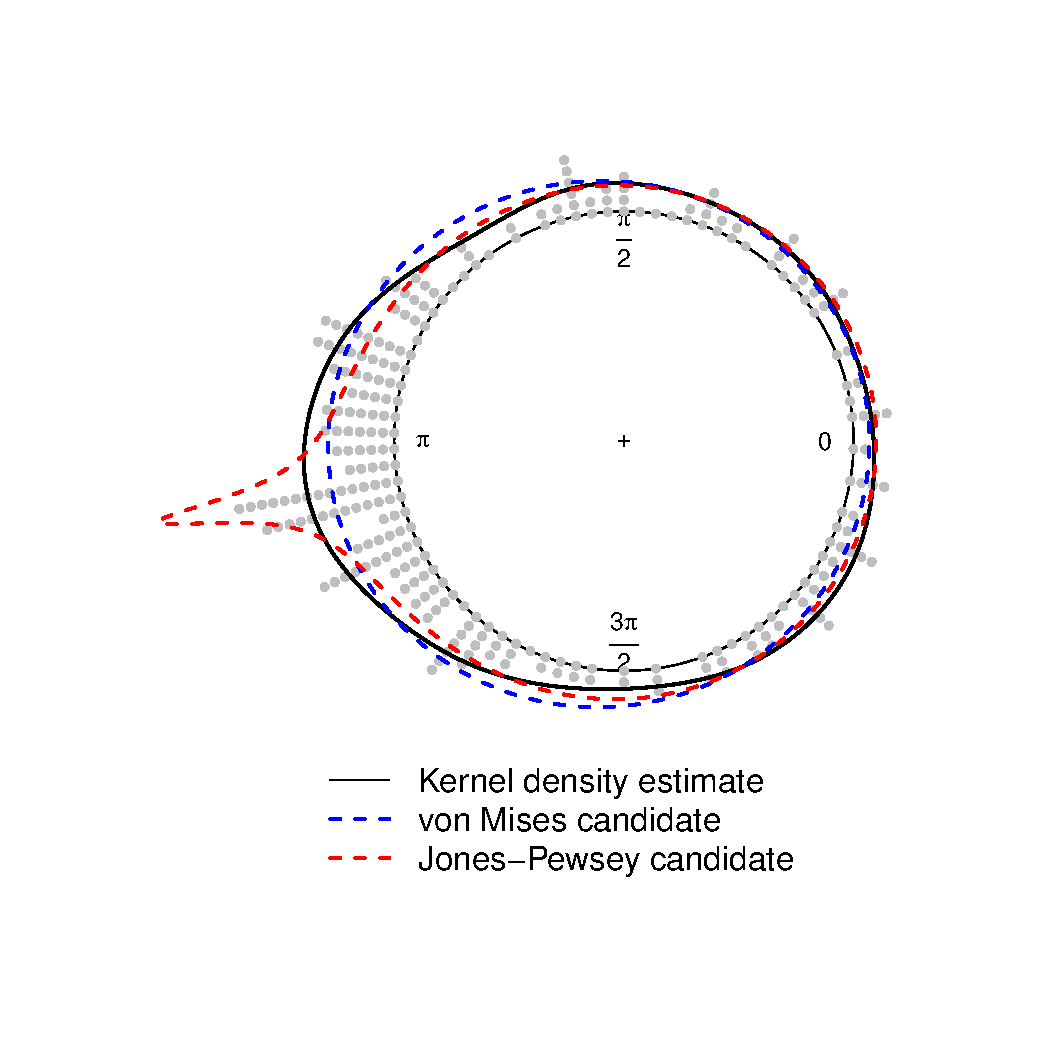
\includegraphics[scale=0.3, keepaspectratio]{plot-mod-pi-2.pdf}
\end{subfigure}
%
\begin{subfigure}[t]{0.5\textwidth}
\caption{Histogram of angles modulo $\pi/2$ with overlaid candidate densities}
\label{fig:linear-density-plot}
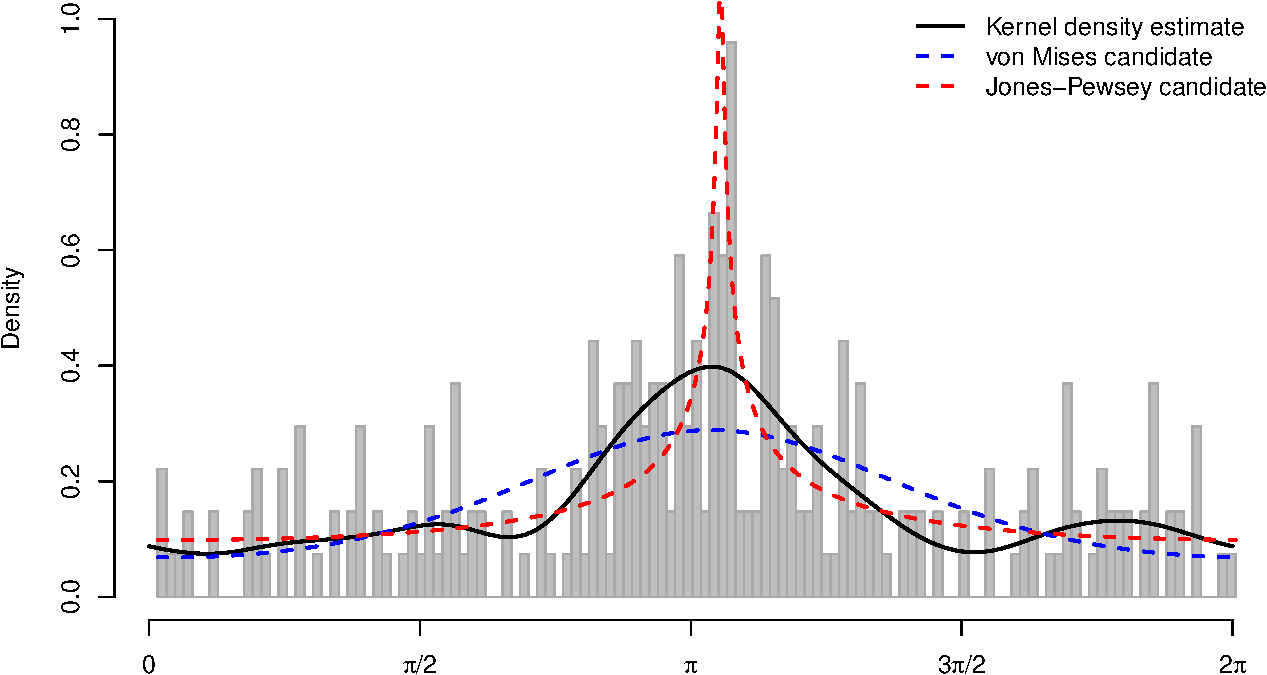
\includegraphics[scale=0.4, keepaspectratio]{linear-density-plot.pdf}
\end{subfigure}
\end{figure}

In fact, the shape of the Jones-Pewsey distribution fitted seems intuitively appropriate for the hypothesis that a substantial subset of the measured angles are `aiming for' a particular bearing, with relatively small symmetric random deviations. The next steps should be to investigate to what degree this is really the case, by fitting a distribution to the angles between points simulated according to this pattern; and to try to identify that subset of the angles that do indeed follow this pattern, as opposed to those that are essentially noise.

\printbibliography

\end{document}